\chapter{Návrh testovací laboratoře}

Pro testování všech výrobků společnosti Conel nejdříve navrhnu strukturu testovací laboratoře.  Testovací laboratoř bude síť obsahující všechny výrobky společnosti Conel, různá příslušenství připojené k jednotlivým výrobkům, testovací server a konfigurovatelné switche.

\section{Testovací server}
Jádrem testovací laboratoře bude server na kterém poběží všechny testovací aplikace. Testovaci server bude výkonější počítač s parametry procesor Intel core i7, 16GB RAM a 512GB SSD disk. Pro účely testování bude server osazen dvěma ethernetovými rozhranímy pro komunikaci s testovanými výrobky a jedním ethernetovým rozhraním pro konektivitu serveru do firemní sítě. Server dále má osazeno jedno WiFi rozhraní pro testování WiFi výrobků.  Operační systém tohoto serveru jsem zvolil Ubuntu server, jelikož operační systém Ubuntu je používán k vývoji většiny výrobků.

Na serveru bude umístěna databáze uchovávající všechny informace o teststování a webová aplikace zobrazující výsledky z testování. Samotná testovací aplikace, včetně testovacích skriptu a příslušného API budou taktéž umístěny na tomto serveru. Dále zde bude kopie vzdáleného repozitáře pro rychlejší stahování zdrojových kódu. V dalších fázích vývoje testovacího zařízení by na temto serveru mohl být testován systém pro monitoring routerů RSeeNet a systém pro jednoduchou tvorbu VPN tunelů SmartCluster.

\begin{figure}[h]
  \centering
  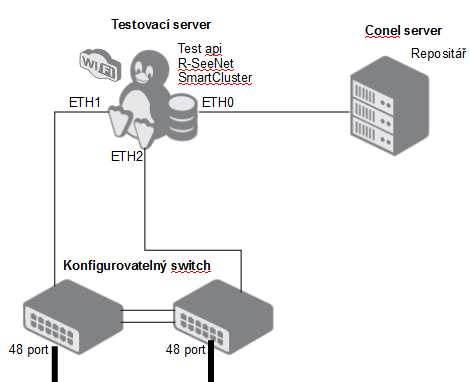
\includegraphics[width=.4\LW]{server_switch}
  \caption{Zapojení testovacího serveru a switchů}
  \label{fig:server_switch}
\end{figure}

\section{Konfigurovatelné switche}
Pro propojení všech výrobků s testovacím serverem budou použity dva konfigurovatelné 48 portové switche od firmy CISCO. Dva switche byly zvoleny kvůli velké ceně switchů nad 48 portů. Konfigurovatelné switch budou potřeba pro změnu síťové infrastruktury v průběhu testu. Každý switch bude připojen k jednomu ethernetovému rozhraní serveru, dále budou switche navzájem propojeny. Nejen všechny výrobky, ale každé fyzické ethernetové rozhraní bude připojeno do switche a pomocí VLAN bude vytvořena požadovaná testovací síť.

\section{Testovaná zařízení}
Zařízení které tvoří přes devadesát procent prodeje firmy Conel jsou bezdrátové routery a i tato zařízení budou testovány v testovací laboratoři. Bezdrátové routery tvoří celkem čtyři modelové řady, které dále obsahují jednotlivé výrobky podle technologie bezdrátového připojení a počtu rozhraní.

\subsection{Řada routerů v0}
Takzvaná nultá řada routerů obsahuje pouze dvá výrobky. Prvním ER75i disponující EDGE technologií, jedním ethernet rozhraním možností a osazením jednoho volitelného portu.  Druhým výrobkem této řady je UR5, který se liší pouze bezdrátovou technologií. Místo EDGE technologie disponuje rychlejší UMTS technologií. Oba tyto výrobky jsou postaveny na uClinuxu a i přes jejich stáří se firmware stále udržuje. U těchto modelů bude testován pouze Lan, který bude připojeni do konfigurovatelného switche. Testování volitelného portu bude popsáno v samostanté kapitole věnující se tomuto problému. Jiné interface tato základní řada nevlastní.

\subsection{Řada routerů v1}
Řada routeru v1 není od nulté řady marketingově ani koncepčně oddělena. Řada je z hlediska vývoje je oddělena jelikož je založena na plnohodnotném Linuxu místo uCLinuxu použitém u předchoích výrobků. Řada obsahuje výrobky UR5i disponující HSPA+ technologií a XR5i, který nedisponuje žádnou bezdrátovou technologií.

\begin{figure}[h]
  \begin{subfigure}[h]{0.5\LW}
    \centering
    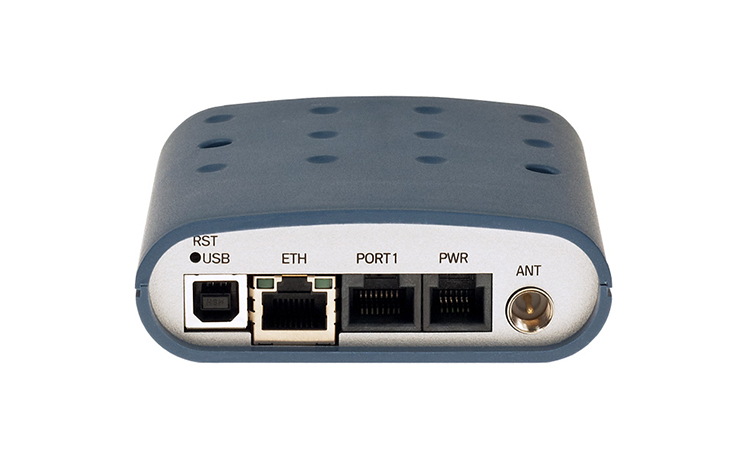
\includegraphics[width=.5\LW]{ER75i}
    \caption{ER75i v plastové krabici.}
    \label{fig:ER75i}
  \end{subfigure}
  \begin{subfigure}[h]{0.5\LW}
    \centering
    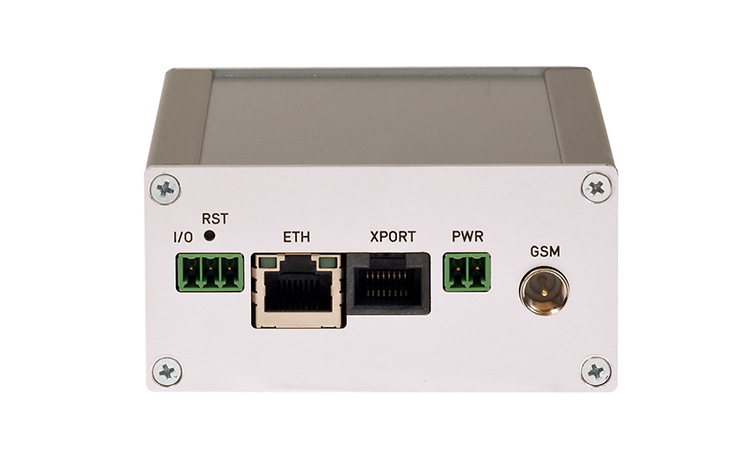
\includegraphics[width=.5\LW]{ER75i_SL}
    \caption{ER75i v kovové krabici.}
    \label{fig:ER75i SL}
  \end{subfigure}
  \caption{Příklad vzhledu řady routerů v0 a v1.}
  \label{fig:ER75i}
\end{figure}

\subsection{Řada routerů v2}
Řada routerů v2 sebou přináší rozsáhlý modulární koncept a tím i velký počet různých typů routerů. Pro pokrytí všech možných kombinací routerů této řady bude muset v testovací laboratoři běžet přibližně třicet routerů. Každý router bude připojen ethernet kabel do konfigurovatelného switche. Vybrané routery budou mít zapojen binární vstup a výstup pro testování vstupů a výstupů. Dále tyto routery budou mít zapojeny různá zařízení do USB konektoru, například flash disk a USB/RS232 převodník. Modelová řada v2 obsahuje taktéž až dva volitelné porty, popis zapojení testování těchto portů bude popsáno v samostné kapitole věnující se volitelným portům.

\begin{figure}[h]
  \begin{subfigure}[h]{0.5\LW}
    \centering
    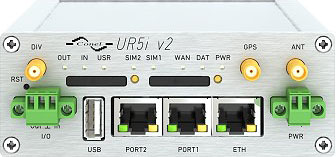
\includegraphics[width=.5\LW]{UR5i_v2}
    \caption{UR5i v2 v kovové krabici.}
    \label{fig:UR5i_v2}
  \end{subfigure}
  \begin{subfigure}[h]{0.5\LW}
    \centering
    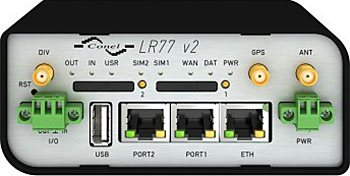
\includegraphics[width=.5\LW]{LR77_v2}
    \caption{LR77 v2 v plastové krabici.}
    \label{fig:LR77_v2}
  \end{subfigure}
  \caption{Příklad vzhledu řady routerů v2.}
  \label{fig:UR5i_v2}
\end{figure}

\subsection{Řada routerů v3}
Modelová řada v3 je poslední vyvinutou řadou routerů. Koncepčně se příliš nelíší od předchozí řady. Různé kombinace routerů lze tvořit pomocí dvou volitelných portů. Jednotlivé porty lze osadit jakýmkoliv volitelným portem, nebo deskou s bezdrátovým modulem. Aby bylo možné obsáhnout testování alespoň nabízených kombinací routerů, bude v testovací laboratoři muset běžet dvacet routerů této řady. V základní konfiguraci bude muset být navíc oproti v2 řadě testován jeden binární vstup a jedno ethernetové rozhraní.

\begin{figure}[h]
  \begin{subfigure}[h]{0.5\LW}
    \centering
    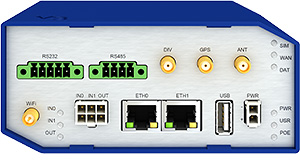
\includegraphics[width=.5\LW]{spectre_LTE}
    \caption{Spectre LTE v plastové krabici.}
    \label{fig:spectre_LTE}
  \end{subfigure}
  \begin{subfigure}[h]{0.5\LW}
    \centering
    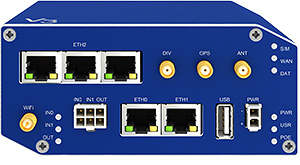
\includegraphics[width=.5\LW]{spectre_LTE_SL}
    \caption{Spectre LTE v kovové krabici.}
    \label{fig:spectre_LTE_SL}
  \end{subfigure}
  \caption{Příklad vzhledu řady routerů v3.}
  \label{fig:spectre_LTE}
\end{figure}

\section{Volitelné porty}
Každý router lze osadit alespoň jedním volitelným portem. Jednotlivé volitelné porty rozšiřují router o další interface. Testován musí být všechny volitelné porty alespoň v každé modelové řadě routerů. Popis volitelných portů a způsob zapojení je popsán v kapitolech týkajících se jednotlivým volitelným portům.

\subsection{Ethernet 10/100}
Volitelný port Ethernet 10/100 rozšiřuje router o další fyzický ethernet. Tento port bude testován stejný způsobem jako základní ethernet na router. Všechny tyto porty budou připojeny do konfigurovatelného switche a pomocí VLAN budou odděleny v jiné síti.

\subsection{RS232}
Volitelný port RS232 rozšiřuje router o standartní sériové rozhraní. Sériová rozhraní budou testována trojím způsobem. Nejdříve budou propojeny dva routery sériovým rozraním a mezi nima budou přenášena data. Drůhým způsobem testů bude připojení loopback desky, která odpovídá na pár jednotlivých komandů. Popis těchto destiček pro všechny rozhraní bude v dalších kapitolách. Poslední testovací případ sériového rozhraní bude připojení libovolného zařízení jiného výrobce se sériovým rozhraním.

\subsection{RS485/RS422}
Volitelný port RS485/RS422 rozšiřuje router o přepínatelné sériové rozhraní RS485 a RS422. Testování těchto portů je identické s rozhraním RS232. Testovat bude potřeba obě tyto rozhraní.

\subsection{M-BUS master}
Volitelný port M-BUS master rozšiřuje router o další typ sériového rozhraní. Testování tohoto portu bude prováděno zapojením M-Bus slave loopback destičky. Druhým způsobem tesování bude zapojení reálného M-Bus měřáku. Reálné zařízení je vždy zapojeno pouze jedno v celém testlabu, do ostatních volitelných portů jsou zapojovány loopback desky.

\subsection{I/O module CNT}
Volitelný port I/O module CNT rozšiřuje router o další binární vstupy, binární výstupy, čítačové vstupy a analogové vstupy. Testování tohoto portu bude prováděno pouze jedním způsobem. Volitelný port CNT se bude testovat pomocí loopback desky CNT.

\subsection{WiFi}
Volitelný port WiFi rozšiřuje router o možnost připojení se do WiFi sítě. Tento rozšiřuící port lze osadit pouze do modelové řady v2. Ŕada routerů v1 nepodporuje WiFi rozhraní. Ŕada routerů v3 má možnost osadit WiFi rozhraní již na zkladní desce. WiFi rozhraní se bude testovat vůči WiFi připojení testovacího routeru, WiFi připojení CISCO routeru a naposledy vůči jinemů Conel routeru s podporou WiFi.

\subsection{SDH}
Volitelný port SDH rozšiřuje možnost routeru o připojení SD karty. Kompatibilita portu SDH je stejná jakou u portu WiFi. Testování portu SDH bude pomocí zápisu a přečtení dat z karty umístěné v držáku SDH portu.

\subsection{Switch}
Volitelný port Switch rozšiřuje možnost připojení až na tři switchované ethernety. Po připojení portu Switch do routeru je první ethernet rozswitchován do všech tří portů. Kompatibilita tohoto volitelného portu je stejná jako u předchozích dvou portů.

\section{Cisco router}
Další důležito součástí testovací sítě je bezdrátový Cisco router. Router je zapojen do testovací sítě pomocí ethernetu. Router dále využívá mobilní a WiFi připojení. Cisco router je součástí testovací sítě z důvodu testování nějakých protokolů oproti jinému referenčnímu routeru. Příklad testovaného protokolu může být IPsec.

\begin{figure}[h]
  \centering
  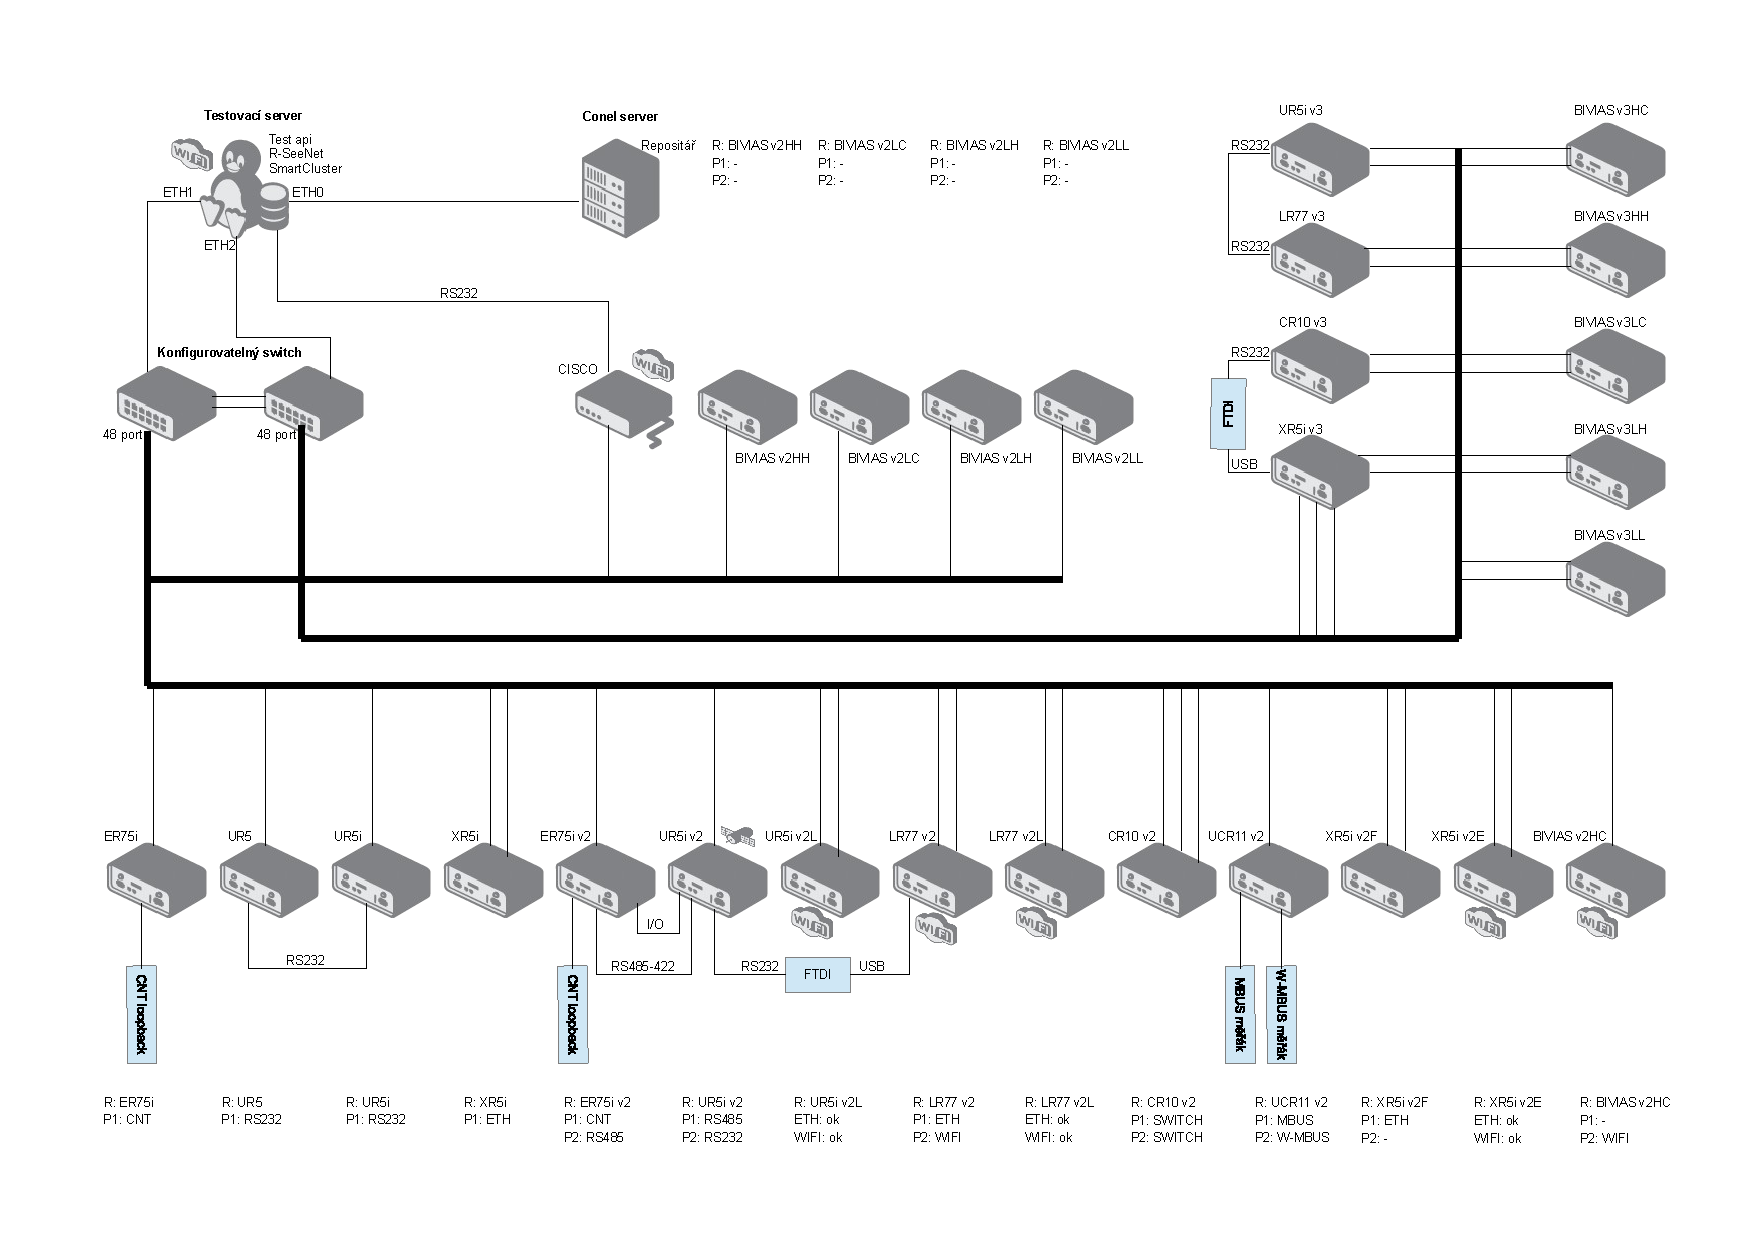
\includegraphics[angle=90,origin=c,width=\LW]{schema_site}
  \caption{Schéma testovací laboratoře}
  \label{fig:schema_site}
\end{figure}

\endinput
